\chapter*{The \cawaqs~platform : general information}
\phantomsection
\addstarredchapter{The \cawaqs~platform : general information}
\fancyhead[LE]{\thepage} 
\fancyhead[RE]{The \cawaqs~platform : general information}
\fancyhead[RO]{\thepage} 
\fancyhead[LO]{The \cawaqs~platform : general information}
\fancyfoot[C]{\thepage}

\renewcommand{\headrulewidth}{0.1pt}

\setlength{\parindent}{0cm} % no indent
\setlength{\parskip}{9pt}
\vspace{-1cm}

% -------------------------------------------------------------

Used in its fullest form, the \cawaqs\ platform computes joint water, solute, and/or energy fluxes within all compartments of a hydrosystem. Conceptually, this model is partly based on the MODCOU software suite \citep{marsily78,ledoux1980}. However, it differs greatly in its structure in integration of the concept of nested scales. In most cases, it is usually divided into three main compartments: sub-surface (\ie~soil compartment), river and/or hydraulic network, vadose and saturated zone (\ie~multi-layered aquifer system), communicating through interfaces. Additional modules and features are also available, which can be required to model more specific types of hydrosystem. To model more complex/unusual systems, the initial structure of the MODCOU software was modularized, rewritten, and coupled according to the concepts of \cawaqs1.X\ \citep{flipo2005} and \cawaqs2.X\ \citep{labarthe2016}, leading to the implementation of the current version of \cawaqs\genversion\ (\version), through a combination of seven main libraries:
\begin{itemize}
    \item \textbf{libfp} (\cref{fig:cawaqs3}-\textbf{A}), which computes surface water balance at a daily time step. This library estimates actual evapotranspiration (AET), evaluates soil water storage, and characterizes infiltration and runoff from total precipitation (\ie\ rain + snow) and potential evapotranspiration (PET) input data. The runoff is then directly transferred to the river network. This conceptualization tends to negate the transfer time between the location of hypodermic runoff generation and the closest river reach. To achieve this, the routing surface mesh defined to transfer runoff consists of elementary catchments, respectively associated with each river reach. Therefore, it is assumed that its routing transfer time is less than the simulation time step (\ie~daily) ;
    \item \textbf{libhyd} (\cref{fig:cawaqs3}-\textbf{B}) computes in-stream river flows using the Muskingum hydrological routing scheme. For each river reach, the associated sub-surface runoff flows are distributed homogeneously along the reach. As a default option, the water level in the stream is calculated as a function of discharge using the Manning-Strickler equation ;
    \item \textbf{libnsat} (\cref{fig:cawaqs3}-\textbf{C}) transfers vertically, in the unsaturated zone (UZ), the infiltrated water flux calculated by the surface module. This transfer is conceptualized by a succession of Nash reservoirs. This compartment introduces a delay in water flow entering the UZ before reaching the outcropping aquifer layers (aquifer recharge) ;
    \item \textbf{libaq} (\cref{fig:cawaqs3}-\textbf{E}) simulates the hydraulic head of a mono- or multilayered aquifer system by solving the diffusivity equation in a pseudo-3D configuration. The equation is solved using a semi-implicit scheme on a squared cells nested meshes ;
    \item \textbf{libttc} (\cref{fig:cawaqs3}-\textbf{F}) solves a generic formulation of the convection/diffusion transport equation. It can be applied to a solute and/or heat transport problem. To solve the transport problem in the river and aquifer compartments, this transport library is coupled to \textit{libhyd} and \textit{libaq} respectively ; 
    \item \textbf{libseb} (\cref{fig:cawaqs3}-\textbf{G}) computes the overall balance of thermal exchanges between water and the atmosphere based on distributed hourly climate data. The balance is composed of four terms: solar radiation (short-wave), long-wave radiation (atmosphere/environment), evapo-condensation (latent heat of phase transition), and convecto-conduction (sensible heat) ;
    \item \textbf{libwet} (\cref{fig:cawaqs3}-\textbf{H}) quantifies the  hydrological balance of lakes (gravel pits) in interaction with the aquifer system while accounting for precipitation, evaporation and runoff. In order to calculate the gravel pit water level, exchanges are estimated according to Darcy's law.
\end{itemize}

\begin{figure}[H]
\begin{centering}
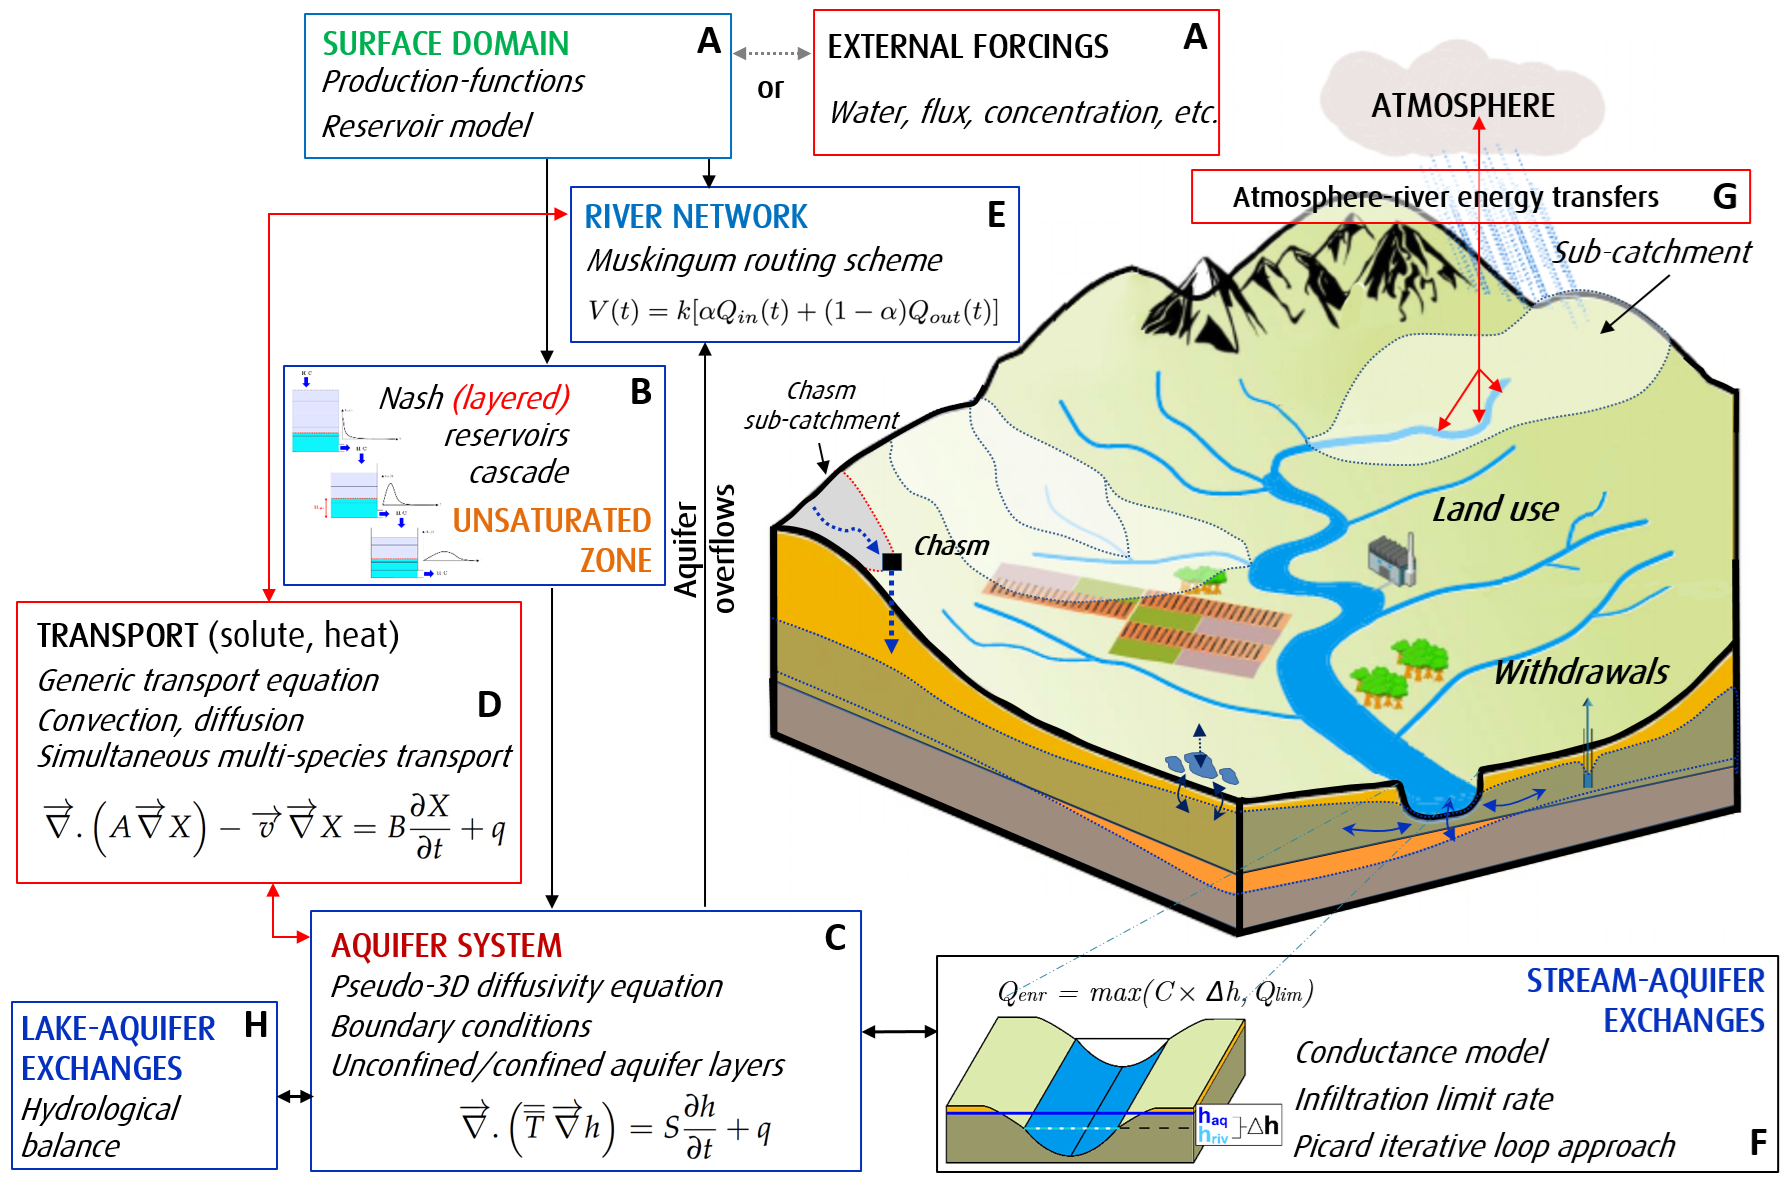
\includegraphics[width=\linewidth]{Figures/Fig_cawaqs3x.png}
\par\end{centering}
\caption[General structure of the \cawaqs\genversion\ hydrosystem modeling platform]{General structure of the \cawaqs\genversion~hydrosystem modeling platform (adapted from \cite{gallois2024} and \cite{flipo2023}). Transport-based features are labeled in red\label{fig:cawaqs3}.}  
\squeezeup
\end{figure}

An optional add-on, known as the "hyperdermal" flow module is available (\cref{sec:HYD-E-hderm}). It introduces a second routing of the simulated output flows exiting the UZ before reaching the aquifer system. This module can be used to simulate runoff flow over deep impermeable bedrocks. This type of runoff is solved through a second use of the Muskingum method.

The \cawaqs\genversion\ modular approach provides the opportunity to activate or disable each compartment according to the user's specific needs or to fit the structure of a particular hydrosystem as closely as possible. In addition, the library-based architecture of the platform gives it considerable scalability.

\cawaqs\ manages flow coupling at the interfaces of the system, especially the groundwater-river exchanges (\cref{fig:cawaqs3}-\textbf{F}). To quantify the stream-aquifer exchange flows, a Picard loop coupled with a conductance model approach is set up. This iterative procedure maintains the semi-implicit scheme to compute exchanged flows between the hydraulic network and the aquifer system, while accounting for a boundary limit rate and drainage of the network. To account for the state of connection of the hydraulic network to the aquifer system, an infiltration limit rate is introduced. This state induces a constant infiltration rate, independent of the hydraulic gradient between the saturated zone and the river.

\cawaqs\ can also be used to account for more unusual types of water flow (hydraulic "short circuits" in an aquifer system - \cref{sec:cascade-aq}). For example, surface chasms can be taken into account, rerouting a fraction of surface runoff into the unsaturated zone. Similarly, discharges from river outlets can be routed to the UZ (\cref{sec:chasm-wb}).

The first part of this guide describes how to run a \cawaqs\,\genversion\ simulation. It also details the structure and content of a command file, as well as its sub-files used to define geometries and parameters of a \cawaqs\ application. Geomatic aspects (\ie\ GIS operations) involved in the construction of the various meshes will not be detailed. The second part details the various conceptual frameworks and associated equations integrated to the \cawaqs\genversion\ platform to account for the physical processes governing water flows and matter/energy transfers within a hydrosystem.